\documentclass[12pt,a4paper,fontset=none]{ctexart}
\usepackage{ctex}
\usepackage{emptypage} 
\usepackage{fancyhdr}
\usepackage{amsmath,amsfonts,amssymb,mathtools}
\usepackage{graphicx}%插入图片用的宏包
\usepackage{mathptmx}
\usepackage{booktabs}
\usepackage[labelfont=bf]{caption}
\usepackage{indentfirst}
\usepackage{caption}
\usepackage{enumitem}
\usepackage[marginal]{footmisc}
\usepackage{subfigure}
\usepackage{fontspec}
\usepackage{geometry}
\usepackage{setspace}
\usepackage{listings}
\usepackage{xcolor}
\usepackage{float}
\usepackage{algorithm,algpseudocode,float}%算法基础宏包
\usepackage{algorithmicx}%算法基础宏包,注意小写
\usepackage{algpseudocode}%算法拓展宏包,函数,Return
\usepackage{lipsum}
\newgeometry{left=3cm,top=2.5cm,bottom=2.5cm,right=3cm}
\setmainfont{Times New Roman}
\setCJKmainfont[BoldFont=SimHei,ItalicFont=KaiTi]{SimSun}
\lstset{
	backgroundcolor=\color{green!10!blue!15},
	rulesepcolor= \color{red!40!blue!100},
	breaklines=true,
	breakatwhitespace=false,
	numbers=left, 
	numberstyle= \small,
	keywordstyle= \color{blue},
	commentstyle=\color{gray}, 
	frame=shadowbox
}
\CTEXsetup[]{section}
\renewcommand{\baselinestretch}{1.5}

\title{\textbf{Problem Set 9}}

\author{
\\
\Large{麻超 \quad 201300066}
\\[6pt]
{ \large \textit{南京大学人工智能学院}}\\[2pt]
}
\date{}

\begin{document}

\maketitle
\setcounter{page}{1}
\section{Problem 1}
\subsection{a}
\begin{figure}[H]
    \centering
    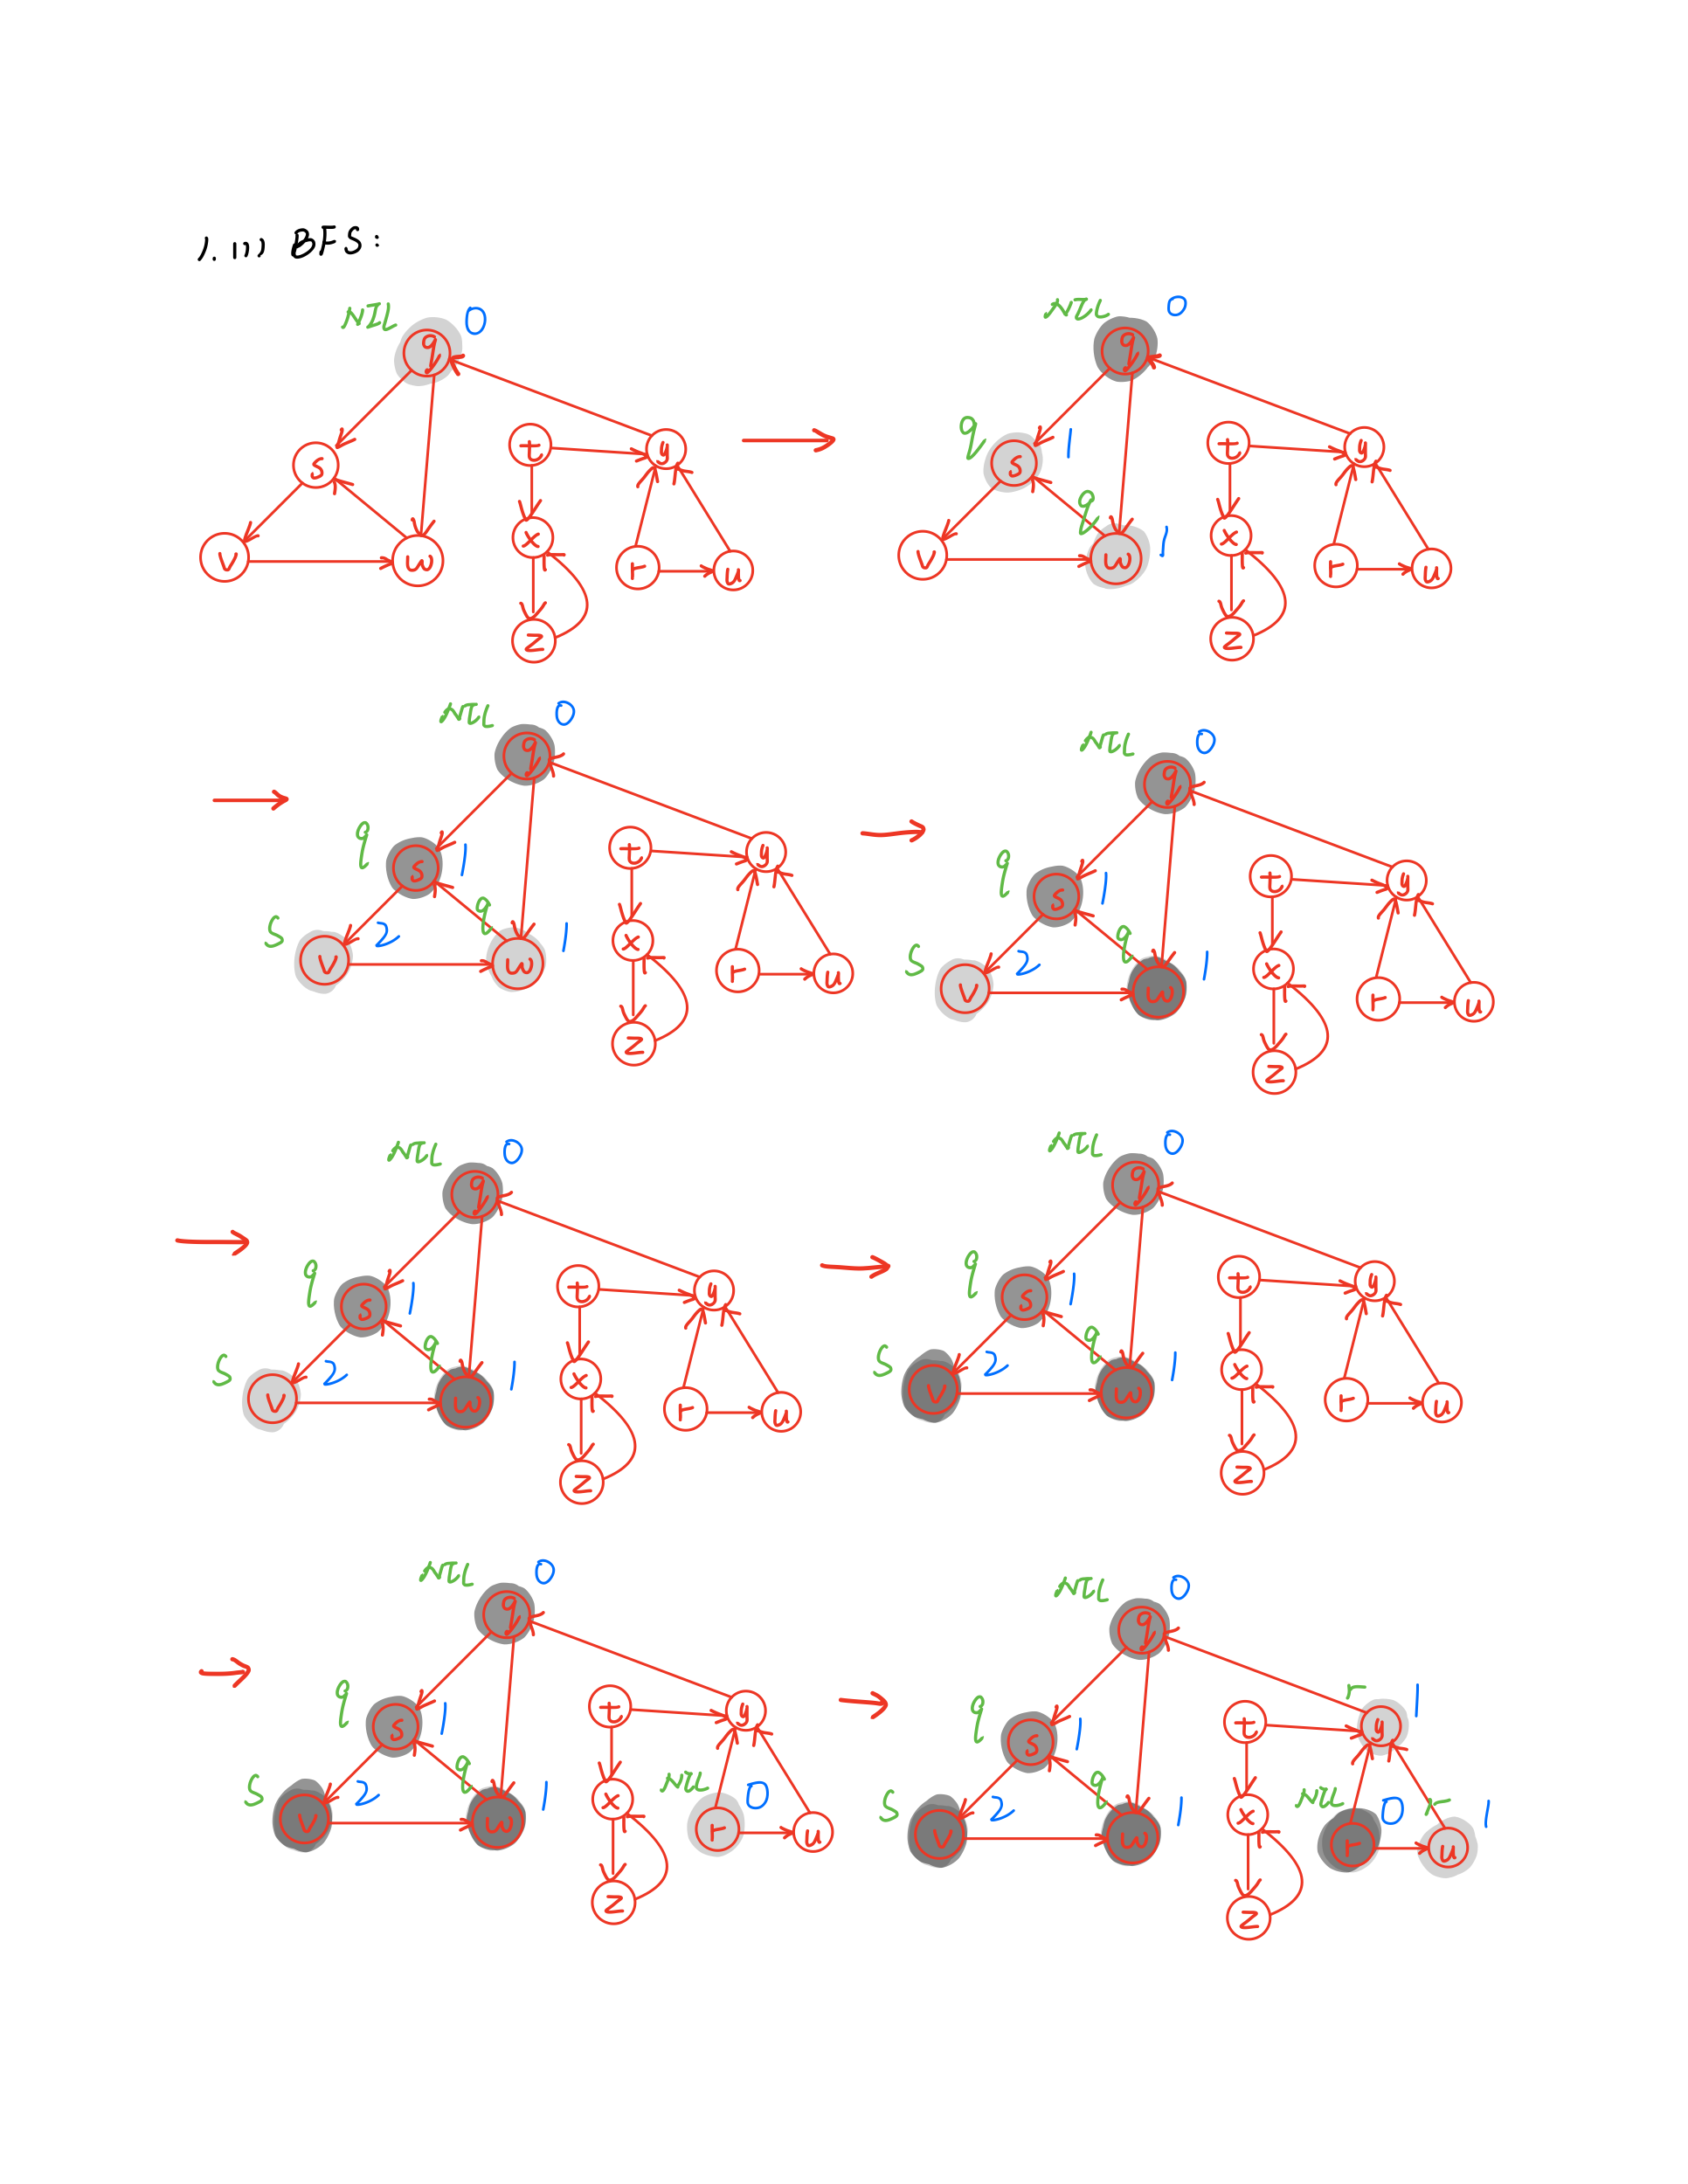
\includegraphics[width=1\linewidth]{IMG_0120.PNG}
\end{figure}
\begin{figure}[H]
    \centering
    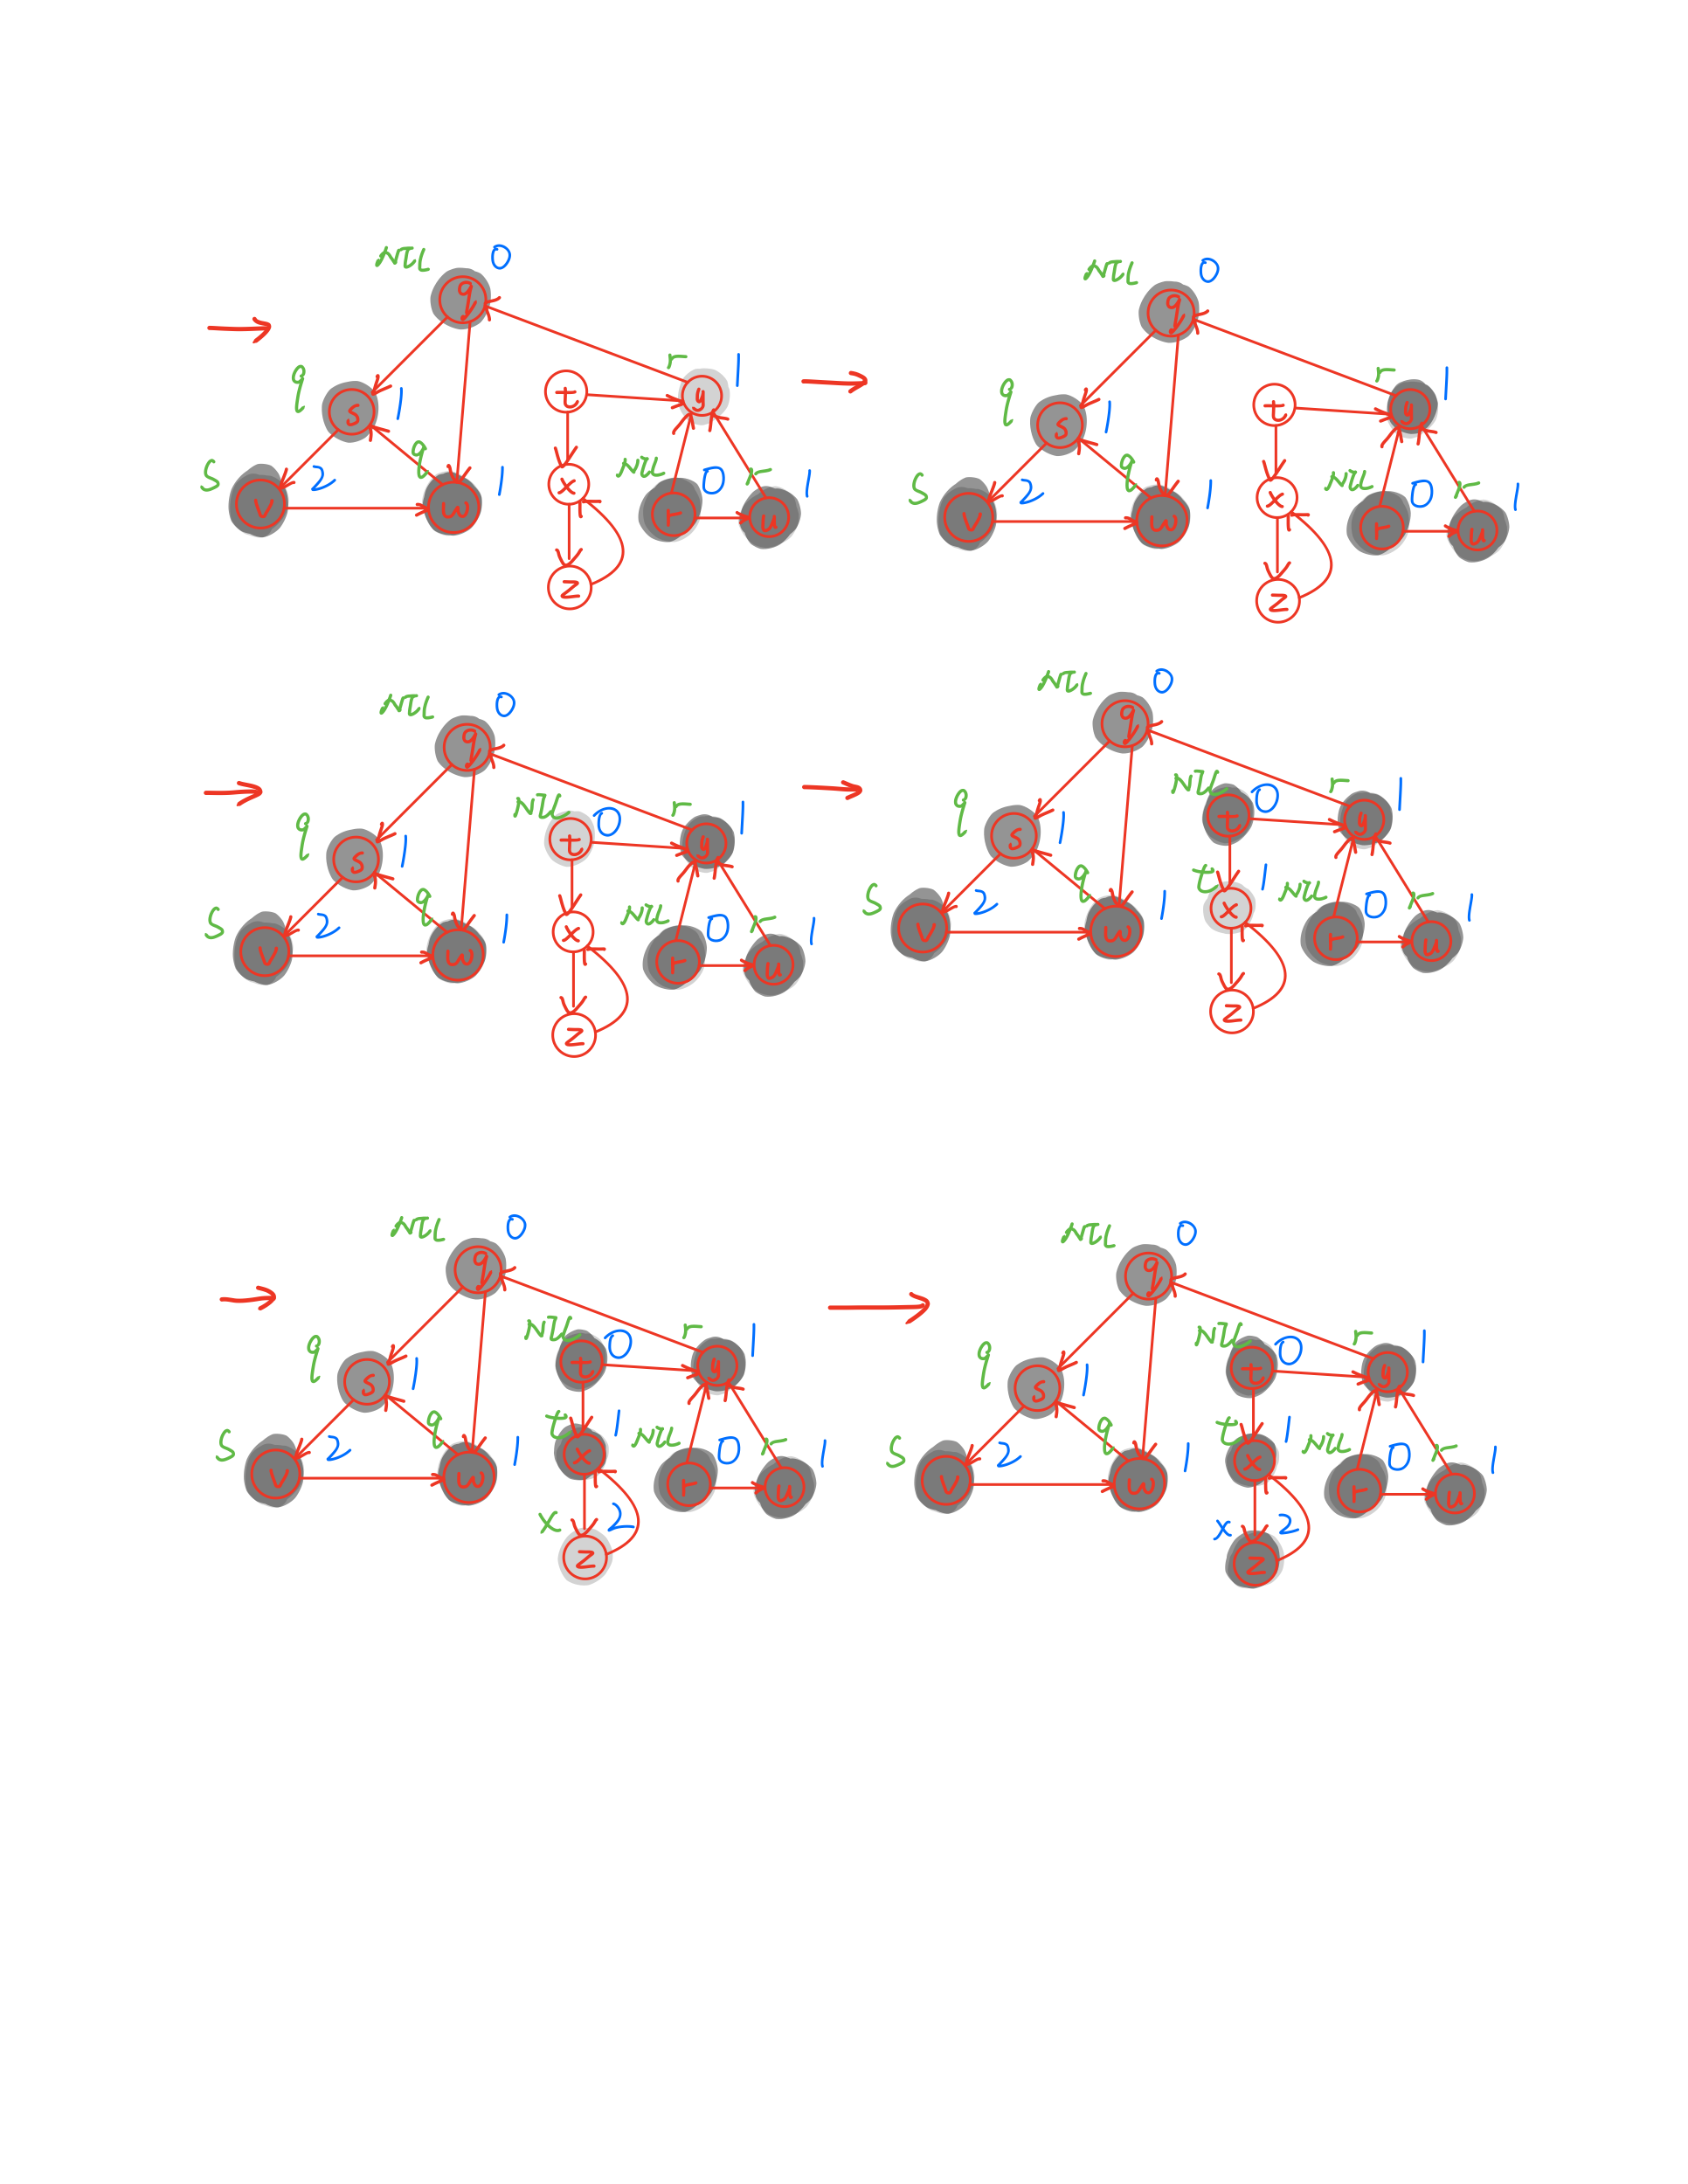
\includegraphics[width=1\linewidth]{IMG_0121.PNG}
\end{figure}
\subsection{b}
\begin{figure}[H]
    \centering
    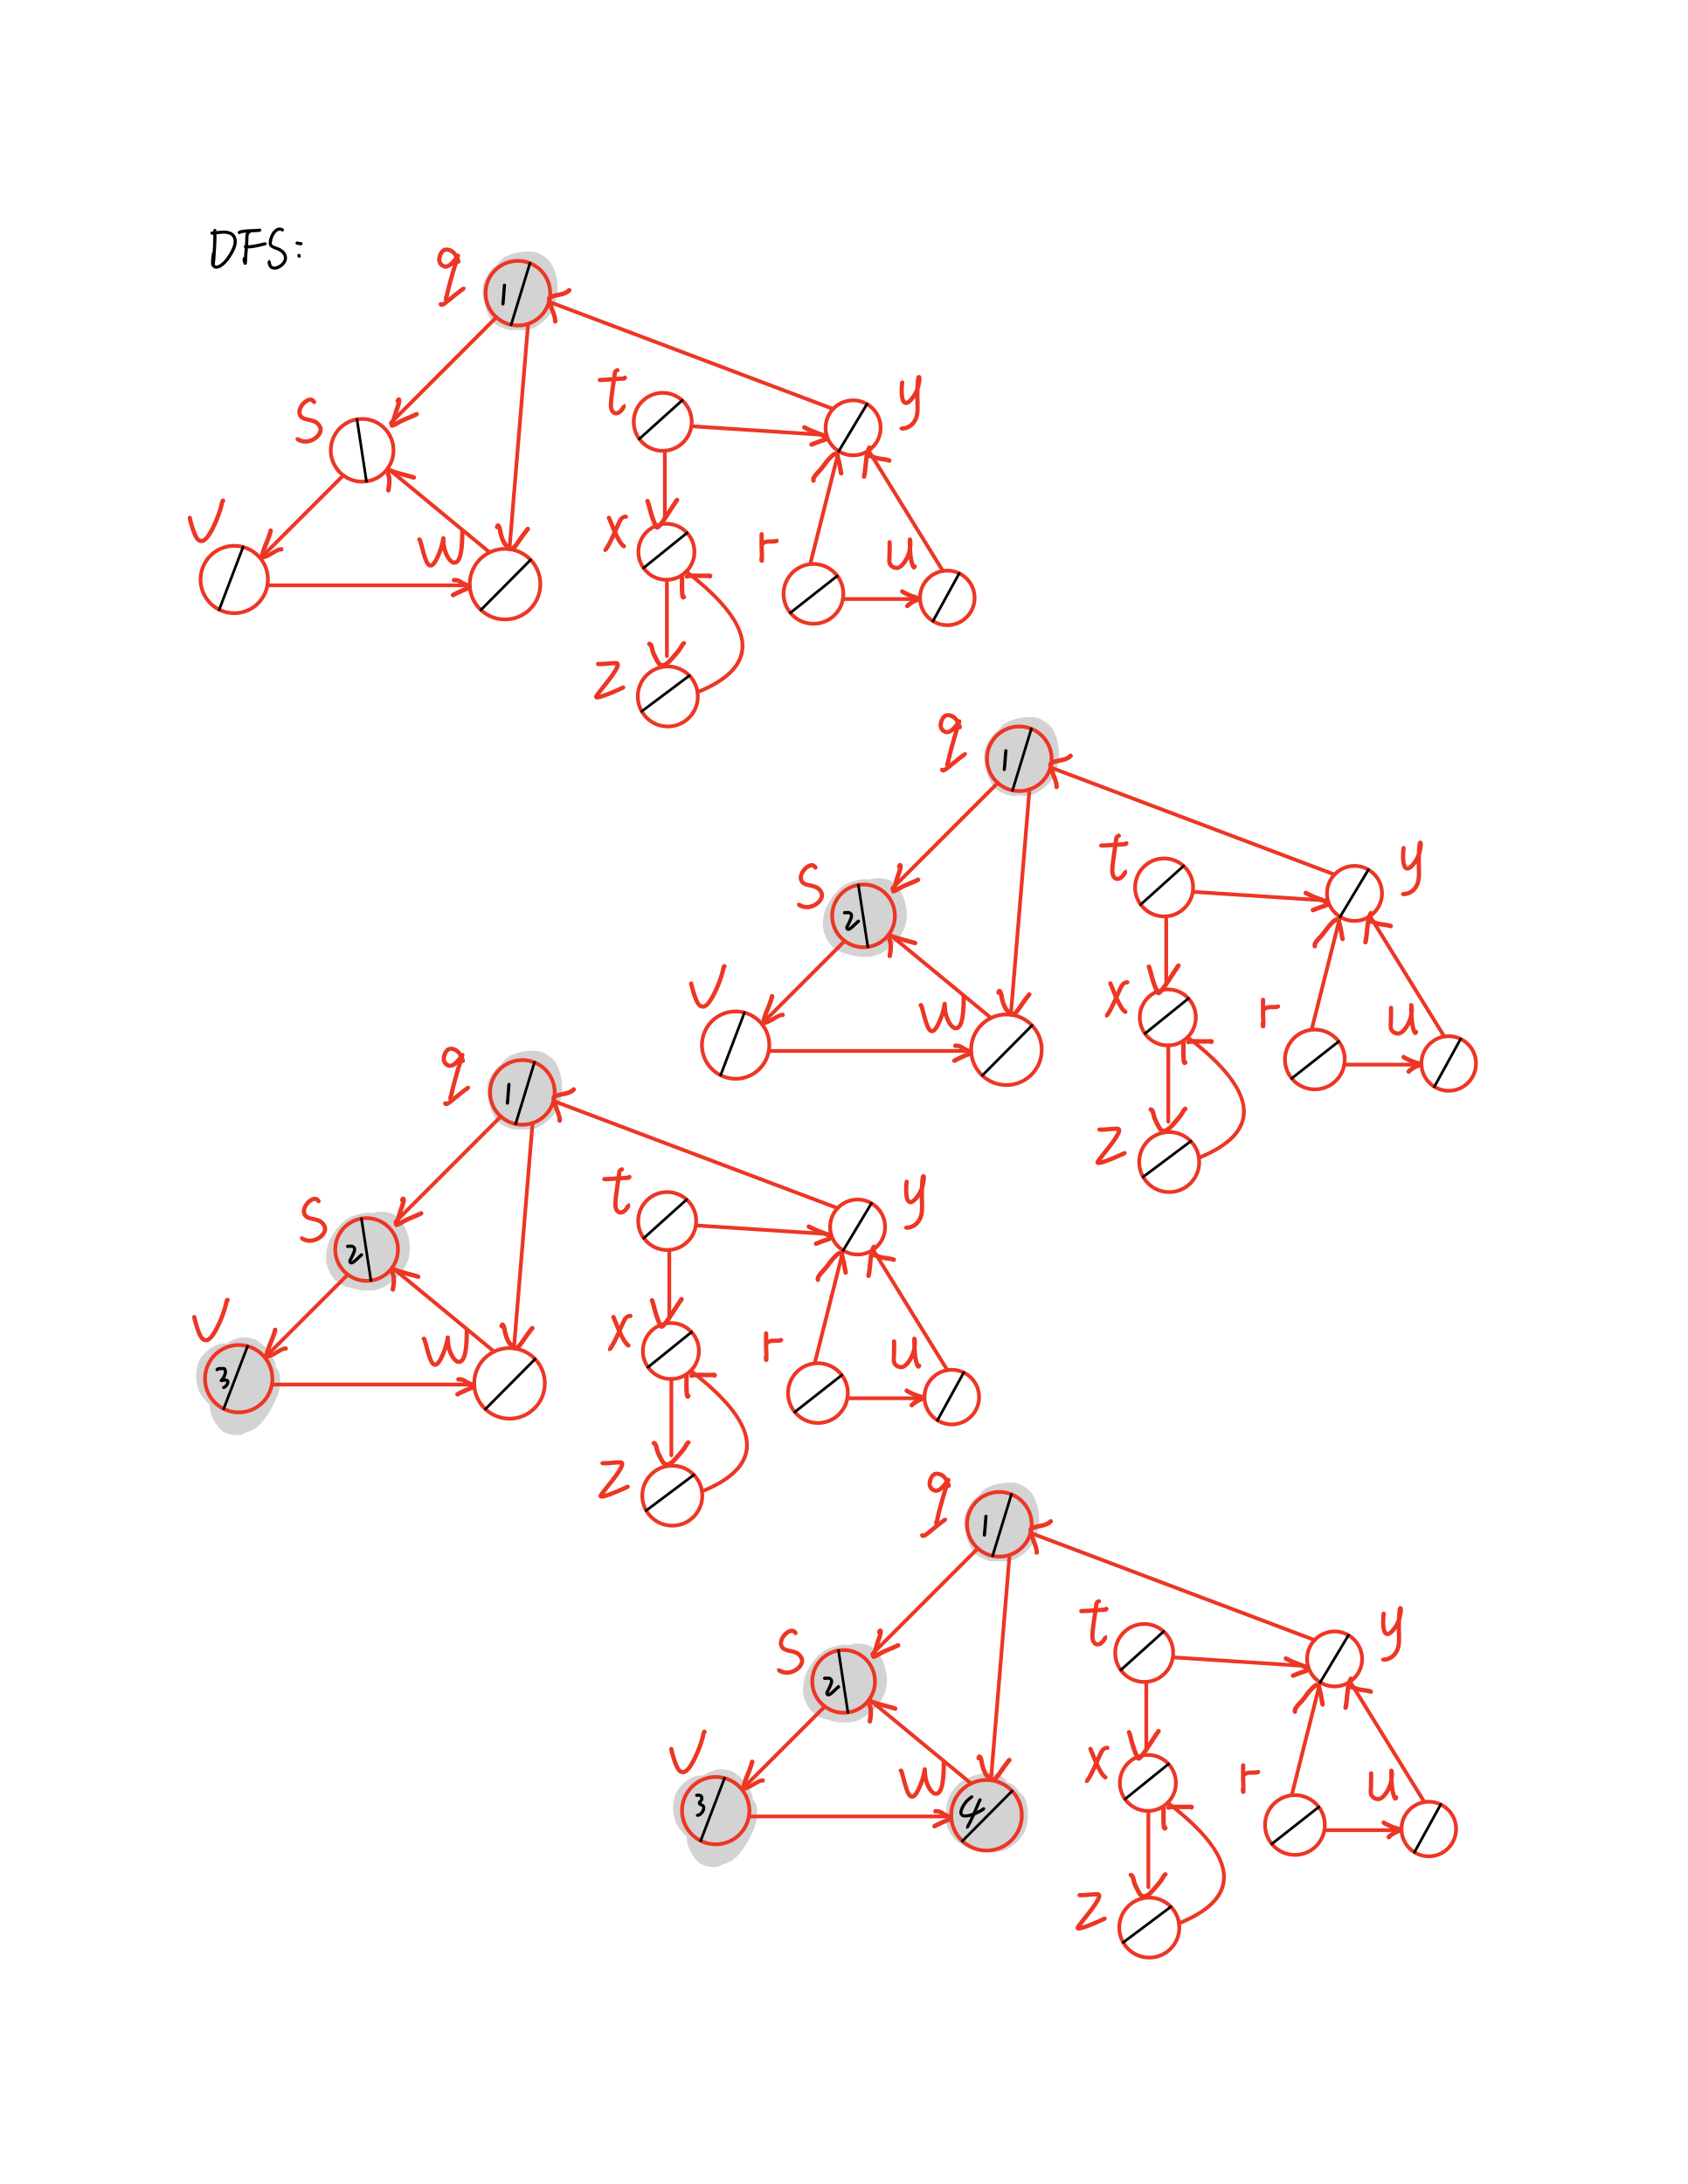
\includegraphics[width=1\linewidth]{IMG_0122.PNG}
\end{figure}
\begin{figure}[H]
    \centering
    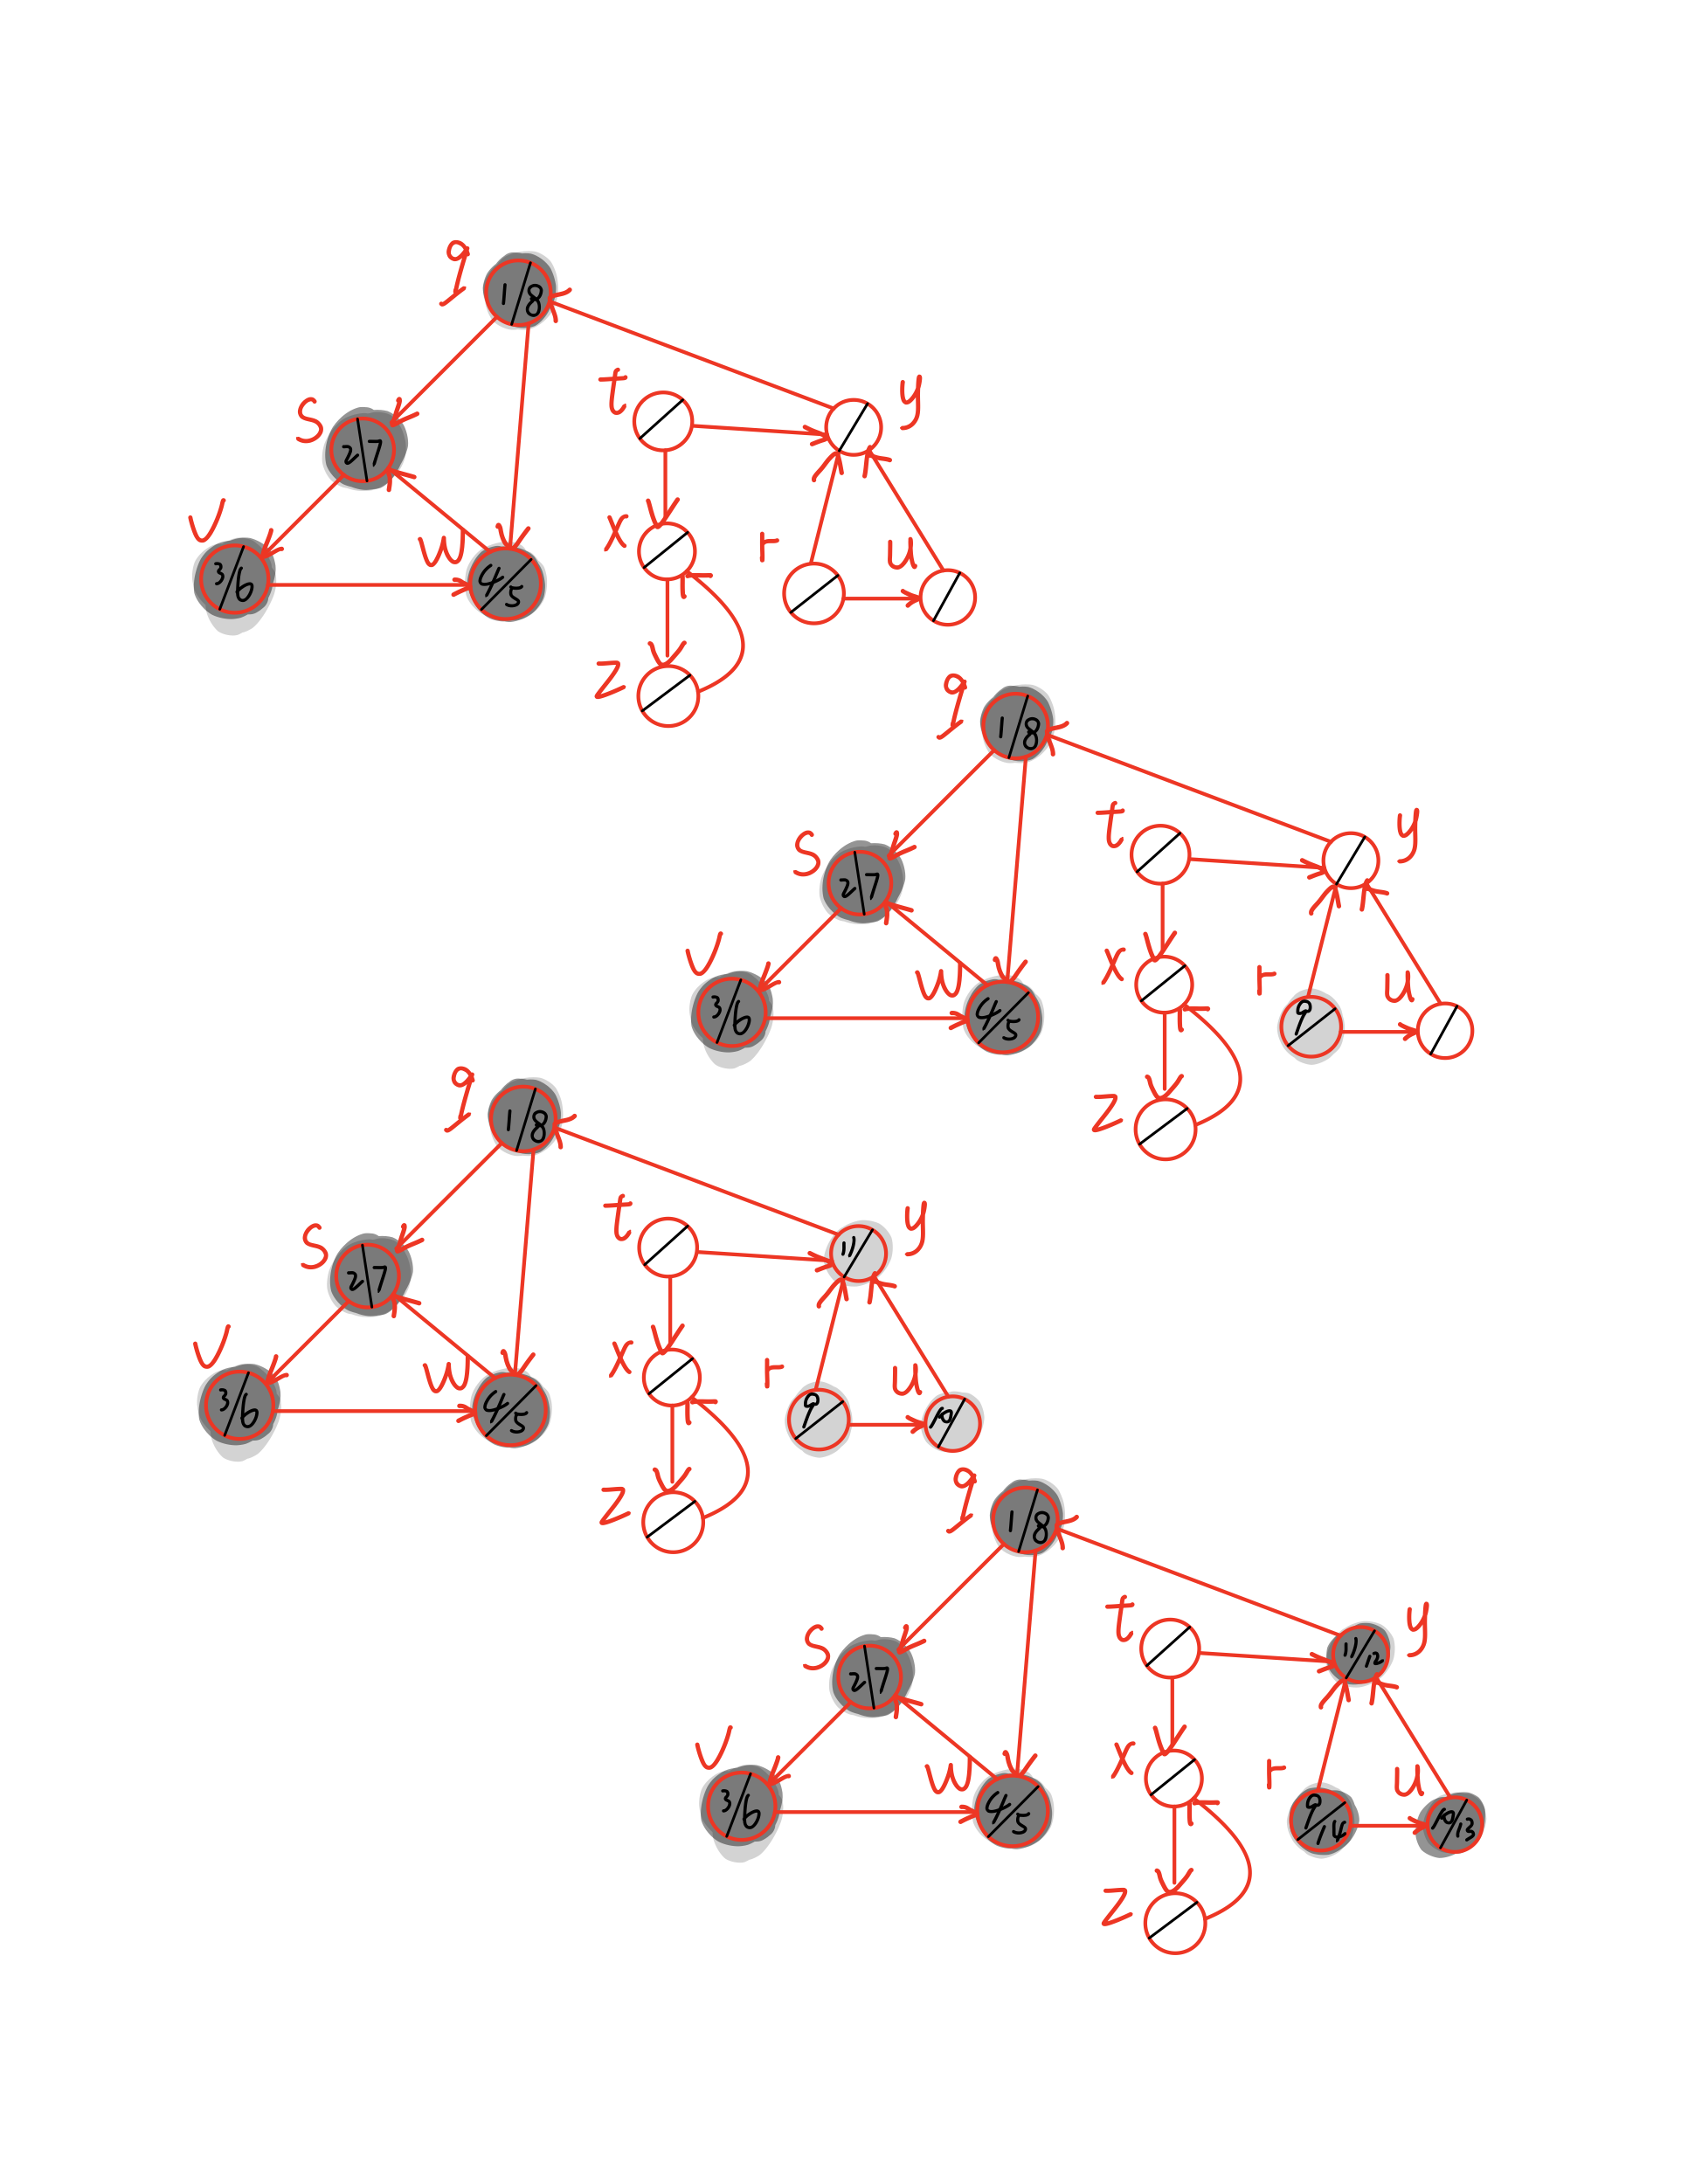
\includegraphics[width=1\linewidth]{IMG_0123.PNG}
\end{figure}
\begin{figure}[H]
    \centering
    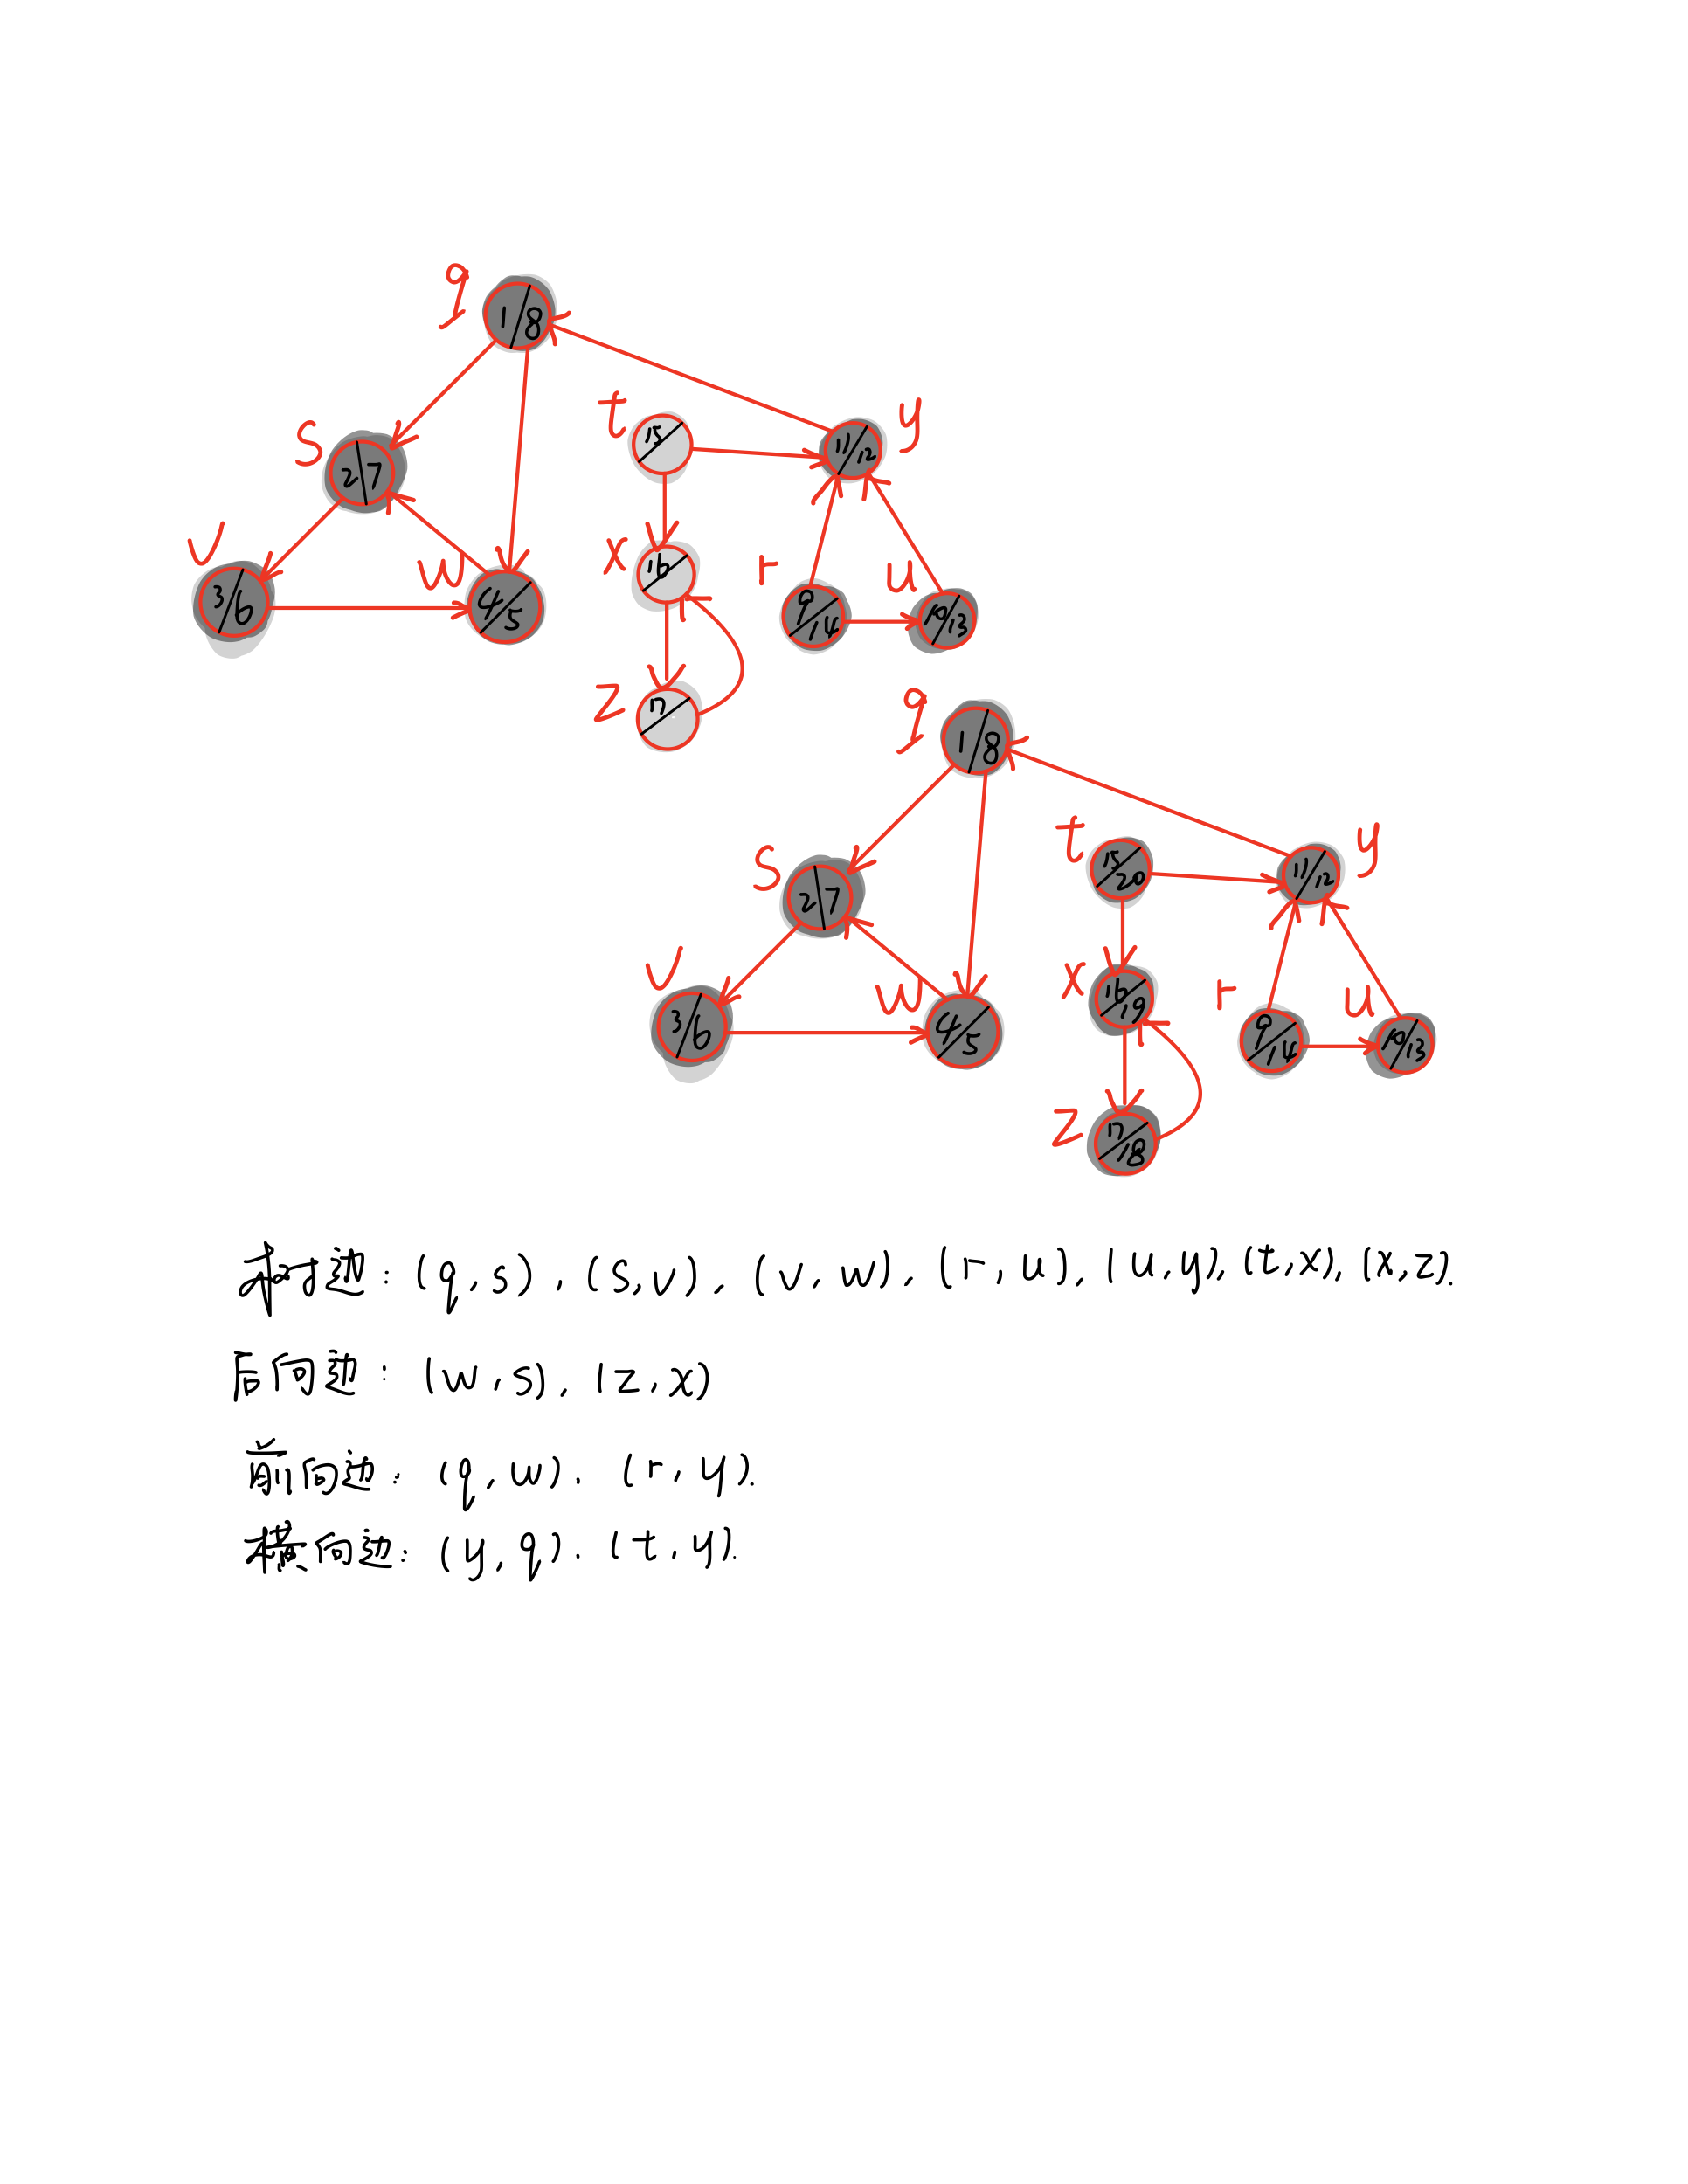
\includegraphics[width=1\linewidth]{IMG_0124.PNG}
\end{figure}
\section{Problem 2}
\subsection{a}
如下图所示,其中s为源顶点,带阴影的边组成一个边的集合$E_{tree}$,自然$E_{tree}$属于E.显然e满足对每一顶点$v\in V$,从s到v的唯一路径是G中的一条最短路径.但是对该图做BFS,无法产生边的集合$E_{tree}$.

假设源顶点s的邻接列表中,顶点u在v之前,那么需要在v之前列出u,自然$w.\pi=u,x.\pi=u$,但这是不成立的.同理,v也不能在u之前,所以对于所有的排列,都不能通过在该图上运行BFS而产生边集$E.{tree}$
\begin{figure}[H]
    \centering
    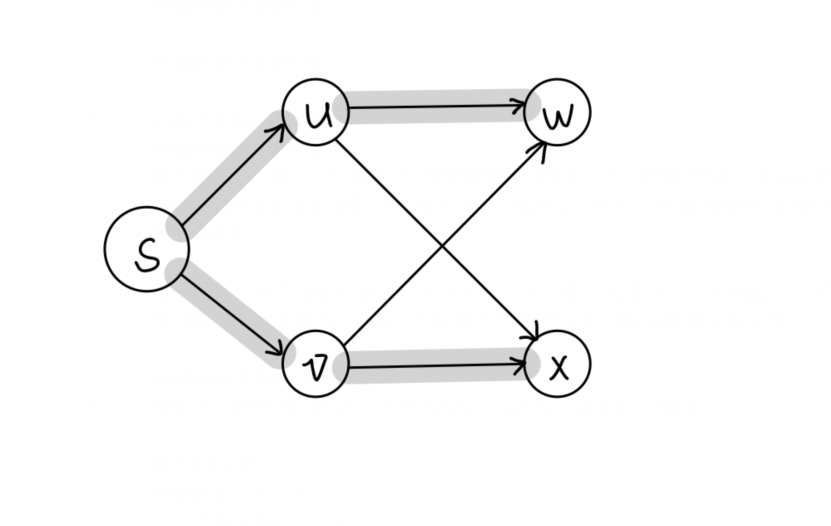
\includegraphics[width=0.7\linewidth]{习题1.png}
\end{figure}
\subsection{b}
按照书上的分类,将边一共分为树边,后向边,前向边,横向边

对于有向图:
\begin{center}
    \begin{tabular}{|c|c|c|c|}
        \hline
        -     & WHITE    & GRAY     & BLACK    \\
        \hline
        WHITE & 所有可能 & 后,横    & 横       \\
        \hline
        GRAY  & 前,横    & 树,后,前 & 树,前,横 \\
        \hline
        BLACK & 横       & 横,后    & 所有可能 \\
        \hline
    \end{tabular}
\end{center}
\subsection{c}
如下图所示,即为反例.
\begin{figure}[H]
    \centering
    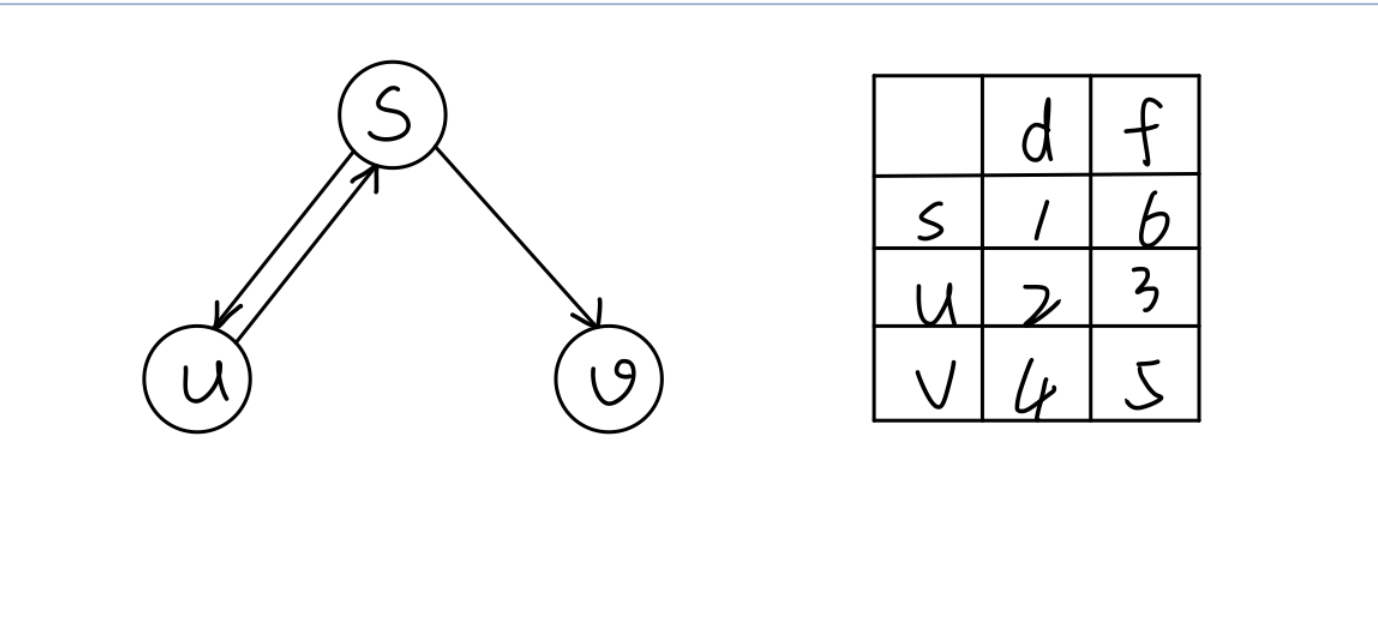
\includegraphics[width=0.7\linewidth]{习题2.png}
\end{figure}
\section{Problem 3}
当执行DFS的第5,6行时,每跳入一次第7行,连通分量数加1,在DFS-VISIT里遇到的结点的联通分量数相同.
\begin{algorithm}
    \renewcommand{\algorithmicensure}{\textbf{Output:}}
    \renewcommand{\algorithmicrequire}{\textbf{Input:}}
    \caption{RE-Dijkstra(G,r,x,y) }
    \label{alg1}
    \begin{algorithmic}
        \State INITIALIZE-SINGLE-SOURCE(G,x)
        \State $S=\emptyset$
        \While{$Q\neq \emptyset$}
        \State $u=$EXTRACT($Q$)
        \State $S=S\cup \{u\}$
        \For {each vertex $v$ if $v \in G.Adj[u]$}
        \If {$v.d<u.d\times r(u,v)$}
        \State $v.d=u.d\times r(u,v)$
        \State $v.\pi =u$
        \EndIf
        \EndFor
        \EndWhile
        \While{$y\neq x$}
        \State Output $y$
        \State $y=y.\pi$
        \EndWhile
        \State Output $x$
    \end{algorithmic}
\end{algorithm}
\begin{algorithm}
    \renewcommand{\algorithmicensure}{\textbf{Output:}}
    \renewcommand{\algorithmicrequire}{\textbf{Input:}}
    \caption{DFS-VISIT(G,u,ceil) }
    \label{alg2}
    \begin{algorithmic}
        \State $time=time+1$
        \State $u.d=time$
        \State $u.color$=GRAY
        \For {each vertex $u\in G:Adj[u]$}
        \If {$v.color$==WHITE}
        \State $v.\pi=u$
        \State DFS-VISIT(G,u,ceil)
        \EndIf
        \EndFor
        \State $u.color$=BLACK
        \State $u.ceil=ceil$
        \State $time=time+1$
        \State $u.f=time$
    \end{algorithmic}
\end{algorithm}
\section{Problem 4}
\subsection{a}
对于每一个树,先找其顶点(根节点),然后与根节点距离为偶数的结点(包含根节点)归为一个点集合,与根节点距离为奇数的结点归为另外一个点集合,那么这两个点集合就构成了图中所有顶点集合的划分.

首先,对于每个树,其节点到根节点的距离是一定的一个整数,则所有的顶点都分属于这两个集合.另外,对于树中的每一条边,其连接的都是分属于两个集合中的顶点,不会连接每个集合内部,则树中所有的边两端的顶点分别属于这两个集合,所以每一个树都是一个二部图.
\subsection{b}
首先证明必要性:

设G为二部图<X,E,Y>.X,Y非空.

设C为G中的任一回路,令C=($v_0,v_1,v_2,...v_{l-1},v_l=v_0$)

由二部图的性质,$v_i$必定相间出现在X和Y中.

设($v_0,v_2,...v_l=v_0$)属于X,($v_1,v-3,...v_{l-1}$)属于Y.则l必然为偶数,即C中有偶数条边.

接下来证明充分性:

设G的所有回路具有偶数长度,并设G为连通图(若G不连通,则可对G的各连通分支作下述讨论):

令G的顶点集为V,边集为E,现构作X,Y,使<X,E,Y> =G.取$v_0$属于V,则令X=\{v|$v=v_0$或到$v_0$有偶数长度的通路\},Y=V-X.

显然,X非空,由于G为一连通图,则$v_0$必然有相邻顶点,则Y亦非空.

假设有一条边(u,v),且u,v都属于X,那么$v_0$有到u偶数长度通路或者$u=v_0$,v同理.无论是哪种情况,均有一条$v_0$到$v_0$的奇数长度的回路,与题设矛盾,所以不可能有这么一条边.Y同理,则没有任何边的两个端点都在X中或都在Y中,因此充分性得证.
\subsection{c}
首先for循环迭代每个点,如果这个点还没有染色,那么就将这个点染色,然后dfs它的所有临点,并且将没有染过色的临点染色成另外一种颜色,如果临点已经染过色了那么判断相邻两点颜色是否一致,一致的话就不是二部图.
\begin{algorithm}
    \renewcommand{\algorithmicensure}{\textbf{Output:}}
    \renewcommand{\algorithmicrequire}{\textbf{Input:}}
    \caption{Judge}
    \label{alg3}
    \begin{algorithmic}
        \State bool flag=true
        \For {$i=1\to n$}
        \If {!color[i]}
        \If {(!dfs(i,1))}
        \State \Return False
        \EndIf
        \EndIf
        \EndFor
        \Function{dfs}{u,c}
        \State {color[u]=c}
        \For {(i=h[u];\~i;i=ne[i])}
        \State {j=e[i]}
        \If{!color[j]}
        \If{!dfs(j,3-c)}
        \Return false
        \EndIf
        \EndIf
        \If {color[j]==c}
        \Return false
        \EndIf
        \EndFor
        \State \Return true
        \EndFunction
    \end{algorithmic}
\end{algorithm}
DFS的时间复杂度为$\Theta(n+m)$,故判断其是不是二部图的时间复杂度为$O(n+m)$.
\section{Problem 5}
选择从迷宫的起点入手推导,利用DFS,当遇到之前已经访问过的节点或者无论这一次怎么走都会出界的节点时就换一条路,如果遍历了所有路径都无法到达终点则说明这个迷宫是无解的,否则则选取所有可到达终点的路径中最短的一条的长度返回.

伪代码如下(下一页):
\begin{algorithm}
    \renewcommand{\algorithmicensure}{\textbf{Output:}}
    \renewcommand{\algorithmicrequire}{\textbf{Input:}}
    \caption{Maze(G,n,point=(1,1))}
    \label{alg4}
    \begin{algorithmic}
        \For {every $v\in G$}
        \State visited[v]=false
        \EndFor
        \State visited[point]=true
        \State nextpoint[]=point.change(point.value)
        \For{every exist point in nextpoint[]}
        \If {point==goal}
        \State \Return pathlength
        \Else \If{point!=visited}
        \State Maze(G,n,point)
        \EndIf
        \EndIf
        \EndFor
    \end{algorithmic}
\end{algorithm}

由于其边和点的总个数不会超过$2n^2$,所以时间复杂度为$O(n^2)$.
\section{Problem 6}
只需要对原图进行一次DFS并注意将符合条件的点纳入即可完成.

伪代码如下:
\begin{algorithm}
    \renewcommand{\algorithmicensure}{\textbf{Output:}}
    \renewcommand{\algorithmicrequire}{\textbf{Input:}}
    \caption{French(G,v)}
    \label{alg5}
    \begin{algorithmic}
        \For {every $v\in G$}
        \State visited[v]=false
        \State result[v]=false
        \EndFor
        \Function{DFS}{G,v}
        \State visited[v]=true
        \State result[v]=true
        \State for each w adjecent to v
        \If {site (w,v) meet the criteria}
        \State result[w]=true
        \If {!visited[w]}
        \State DFS(G,w)
        \EndIf
        \EndIf
        \EndFunction
    \end{algorithmic}
\end{algorithm}

由于DFS的时间复杂度为$\Theta(n+m)$,所以该算法的时间复杂度为$O(n+m)$
\end{document}